\chapter{Prueba de Concepto}
\label{ch:aplicacion}

\begin{quote}
	{\bf\textsc{Resumen:}} Este capítulo presenta la prueba de concepto realizada para la incorporación de Información Geográfica, procedente de Ogíjares (Granada), mediante herramientas de la Web Semántica. En el ejemplo se estudian y proponen herramientas de la Web Semántica que se pueden utilizar para representar e integrar datos geoespaciales con diferentes geometrías.
\end{quote}



\section{Web Semántica Geoespacial}

Como hemos comentado, uno de nuestros objetivos es estudiar las herramientas de la Web Semántica que se pueden utilizar para representar e incorporar Información Geográfica, valorarlas y desarrollar una prueba de concepto. Para ello es necesario haber entendido los capítulos dedicados a los sistemas SIG y a la Web Semántica, y así comprender que el principal nexo de unión entre ambas tecnologías se obtiene a través de las consultas realizadas con GeoSPARQL. Sabiendo todos estos conocimientos es posible comenzar con el desarollo de la ontología, sin embargo, la primera tarea imprescindible es la selección del conjunto de datos geoespaciales que se desea hacer accesible mediante la Web Semántica. \\

Durante la prueba de concepto contaremos con la presencia de las herramientas destinadas a la generación de información geoespacial (\texttt{QGIS} para permitir obtener la información de los \textit{Shapefile} a hojas de cálculo), generación de documentos \textit{RDF}  (\texttt{Protegé} para permitir llevar la información de los \textit{Shapefile} hacia documentos en formato \textit{RDF} de manera gráfica y su posterior visualización), consumo (\texttt{GraphBD} para permitir la visualización de archivos en formato \textit{RDF} y la realización de las consultas del lenguaje estándar de consulta geoespacial \textit{GEOSPARQL}) y visualización de la información geoespacial obtenida de las consultas (\texttt{R} para permitir ubicar la información geográfica en un mapa interactivo mediante la librería \textit{Shiny}). 

\textit{\textbf{Nota}: La versión usada de QGIS es la 3.8.0-Zanzibar para macOS 10.14}

\subsection{Selección y obtención de los datos geográficos}

En la actualidad, disponemos de diversas fuentes oficiales y no oficiales que nos proporcionan mapas de calidad con los que poder trabajar. No obstante, al querer hacer uso de Información Geográfica de España, es importante destacar dos fuentes principales:

\begin{itemize}
	\item \textbf{Instituto Geográfico Nacional (IGN)}, es la fuenta oficial para todo el territorio español y la descarga de mapas se puede realizar a través de la dirección \url{http://centrodedescargas.cnig.es/CentroDescargas/buscador.do#}.
	
	\item \textbf{Instituto de Estadística y Cartografía de Andalucía}, es la fuente oficial para todo el territorio andaluz y la descarga de mapas se puede realizar a través de la dirección \url{https://www.juntadeandalucia.es/institutodeestadisticaycartografia/bcadescargas/}.
\end{itemize}
 
Sin embargo, como vamos a trabajar con datos procedentes de la provincia de Granada, en concreto de mi pueblo Ogíjares, he optado por escoger los que nos proporciona el \textit{Instituto de Estadística y Cartografía de Andalucía} \cite{base-andalucia}. A continuación, se muestran los pasos para su obtención:

\begin{enumerate}
	\item La descarga se realiza a través de la plataforma del Instituto de Estadística y Cartografía de Andalucía, de la Consejería de Economía y Conocimiento (URL mencionada en el punto anterior). Una vez dentro, seleccionamos la opción \textit{Base Cartográfica de Andalucía (2)}, escogemos \textit{Base Cartográfica de Andalucía (shape)} y buscamos el municipio de \textit{Ogíjares} (figura \ref{fig:obtencion-informacion}). Nos aparecerán varios cuadrantes, escogemos con el que nosotros queramos trabajar; yo me he descargado el cuadrante que aparece seleccionado y remarcado en color.
	
	\begin{figure}[H]
		\centering
		\includegraphics[width=1\linewidth]{imagenes/capitulo4/obtencion-informacion}
		\caption{Portal del Instituto de Estadística y Cartografía}
		\label{fig:obtencion-informacion}
	\end{figure}

	\item La carpeta descargada contiene mapas de áreas muy diversas, las cuales hacen uso de geometría de punto, de línea o de área. Entre las capas que se nos proporciona nos podemos encontrar diversos modelos de datos (tabla \ref{elementos-mapas}). \textit{Si queremos saber más sobre de cada uno de ellos debemos acceder al siguiente \underline{\href{https://www.juntadeandalucia.es/institutodeestadisticaycartografia/prodCartografia/bc/modelo/00_Modelo_Datos_Base_Cartografica_Andalucia.pdf}{enlace}}.}
	
	
	
	\begin{table}[H]
		\caption{Esquema del modelo de datos descargado}
		\label{elementos-mapas}
		\centering
		\begin{tabular}{|m{6.2cm}|m{5.4cm}|}
			\hline
			\rowcolor[HTML]{EFEFEF} 
			\textbf{MODELO DE DATOS} & \textbf{ELEMENTOS} \\ \hline
			\textsc{Infraestructuras geográficas}&   Puntos geodésicos, líneas administrativas            \\ \hline
			\textsc{Toponimia}&              Topónimos      \\ \hline
			\textsc{Relieve}&         Curvas de nivel, puntos de cota           \\ \hline
			\textsc{Sistema urbano}&       Edificaciones, curvas artificiales             \\ \hline
			\textsc{Servicios}&       Centros educativos, instalaciones deportivas             \\ \hline
			\textsc{Red hidrográfica}&       Corriente artificial, punto fluvial  \\ \hline
			\textsc{Red viaria}&      Carreteras, carril bici              \\ \hline
			\textsc{Infraestructuras energéticas y de telecomunicaciones}&     Instalación de energía eléctrica, explotación minera               \\ \hline
			\textsc{Infraestructuras hidráulicas}&     Deósitos hidráulicos, presa               \\ \hline
			\textsc{Infraestructuras de transportes} &         Área de servicio de descanso       \\ \hline
			\textsc{Infraestructuras medioambientales} &     Instalación de tratamiento de aguas.               \\ \hline
			\textsc{Cubierta terrestre}&           Lindes        \\ \hline
		\end{tabular}
	\end{table}
	
	\begin{figure}[H]
		\centering
		\includegraphics[width=1\linewidth]{imagenes/capitulo2/shapefile}
		\caption{Diferentes archivos que componen el formato Shapefile }
		\label{fig:shapefile}
	\end{figure}
	
	\item El fichero descargado para cada uno de los modelos de datos que acabamos de comentar tiene como formato principal \textit{Shapefile (sh)}, el formato más usado para almacenar información geoespacial. Es un formato de archivos que almacena información no topológica con características espaciales de elementos geográficos que soportan geometrías como puntos, líneas y polígonos \cite{tesis}.  Es originario de \textit{Enviromental Systems Research Institute} (ESRI)\footnote{Empresa que desarolla y comercializa software para SIG.} y consta fundamentalmente de un archivo principal, un archivo de índice y una tabla dBase. Estos archivos suelen requerir poco espacio de almacenamiento en disco y se pueden leer y escribir con facilidad. Los diferentes archivos que componen el formato Shapefile tienen el mismo nombre cada uno con su respectiva extensión, como se aprecia en la figura \ref{fig:shapefile}:
	

	\begin{itemize}
		\item \textbf{Archivo principal (*.shp)}: archivo de longitud variable en el que cada registro describe una forma con sus respectivos vértices. 
		
		\item \textbf{Archivo de índice (*.shx)}: acompaña al archivo principal (*.shp) que almacena la posición de los identificadores de entidades individuales en el archivo .shp 
		
		\item \textbf{Tabla dBase (*.dbf)}: almacena la información de atributos de las entidades. 
	\end{itemize}	

	\item La visualización del archivo Shapefile se puede realizar a través de cualquier software GIS, en nuestro caso vamos a utilizar el software de análisis geoespacial QGIS. Respecto los modelos de datos disponibles que se desean escoger para hacer accesible mediante la Web Semántica, vamos a centrarnos en la información geoespacial de edificaciones, curvas de nivel y cotas de altura de Ogíjares (Granada) \cite{info-sh}:
	
	\begin{figure}[H]
		\centering
		\includegraphics[width=0.7\linewidth]{imagenes/capitulo4/codificacion}
		\caption{}
		\label{fig:codificacion}
	\end{figure}
	

		\begin{figure}[H]
		\centering
		\includegraphics[width=1\linewidth]{imagenes/capitulo4/edificaciones}
		\caption{Visualización del elemento \textit{Edificaciones} en QGIS}
		\label{fig:edificaciones}
	\end{figure}

	\begin{itemize}
		\item \textbf{Edificaciones}: se agrupan en esta capa varios elementos que conforman edificaciones con geometría de polígono (figura \ref{fig:edificaciones}). Dispone de la información:
		
		\begin{itemize}
			\item \textsc{GID}.	
			\item \textsc{ID de la hoja}.
			\item \textsc{Estado}: estado de uso de la entidad o el tramo de la entidad.
			\begin{itemize}
				\item 	\small{En construcción (CON), en ruinas (RUI), sin clasificar (SCL) o en uso (USO).}
			\end{itemize}
			
			\item \textsc{Tipo}: tipo de elemento según su función.
			\begin{itemize}
				\item 	\small{Caseta o cobertizo (CAS), caso genérico (CGN), chabola (CHA), chimenea (CHI), edificación (EDI), industrial (IND), invernadero (INV), marquesina (MAR), nave abierta (NAB), nicho (NIC), patio (PAT), sin clasificar (SCL), tentadero (TEN), torre genérica (TGN), transformador (TRF) o torre de vigía (TVG).}
			\end{itemize}
			 
		\end{itemize}

		\begin{figure}[H]
			\centering
			\includegraphics[width=1\linewidth]{imagenes/capitulo4/curvasnivel}
			\caption{Visualización del elemento \textit{Curvas de Nivel} en QGIS}
			\label{fig:curvasnivel}
		\end{figure}
		
		\item \textbf{Curvas de nivel}: línea imaginaria de altitud constante que sirve para describir la forma tridimensional de la superficie terrestre con geometría de línea (figura \ref{fig:curvasnivel}). Dispone de la información:
		
		\begin{itemize}
			\item \textsc{GID}.	
			\item \textsc{ID de la hoja}.
			\item \textsc{Cota}: recoge la coordenada altura ortométrica del elemento capturado en metros.
			\item \textsc{Categoría}: categoría de la curva de nivel.
			\begin{itemize}
				\item 	\small{Auxiliar (AUX), maestra (MAE), normal (NOR) o sin clasificar (SCL).}
			\end{itemize}
			
			\item \textsc{Procedencia}: procedencia de la curva de nivel.
			\begin{itemize}
				\item 	\small{Combinado (CMB), elementos terreno (ETE), lidar (LID), MDT (MDT), restitución (RES) o sin clasificar (SCL).}
			\end{itemize} 
			\item \textsc{Tipo}: tipo de la curva de nivel.
			\begin{itemize}
				\item 	\small{Caso genérico (CGN), depresión (DEP) o sin clasificar (SCL).}
			\end{itemize}
			
		\end{itemize}
	

		
		
		\begin{figure}[H]
			\centering
			\includegraphics[width=1\linewidth]{imagenes/capitulo4/puntocota}
			\caption{Visualización del elemento \textit{Punto Cota} en QGIS}
			\label{fig:puntocota}
		\end{figure}
		
		\item \textbf{Punto cota}: punto situado sobre la superficie terrestre del cual se conoce su altitud sobre el nivel medio del mar, y que se representa para facilitar la interpretación gráfica de la morfología del terreno con geometría de punto (figura \ref{fig:puntocota}). Dispone de la información:
		
		\begin{itemize}
			\item \textsc{GID}.	
			\item \textsc{ID de la hoja}.
			\item \textsc{Cota}: recoge la coordenada altura ortométrica del elemento capturado en metros.
			\item \textsc{Contexto}: contexto del punto de cota.
			\begin{itemize}
				\item 	\small{Caso genérico (CGN), cima (CIM), collado (COL), depresión (DEP), edificación (EDI) o sin clasificar (SCL).}
			\end{itemize}
		\end{itemize}

		\item \textsc{Tipo}: tipo de elemento según su función.
		
		\begin{itemize}
			\small{
			\item Punto cota construcción elevada (CON) o punto cota terreno (TER).
		}\end{itemize}
	\end{itemize}

\end{enumerate}

Con esto hemos terminado de explicar los datos que vamos hacer accesibles a través de la Web Semántica. En la figura \ref{fig:mapa} es posible visualizar las tres geometrías juntas y localizadas en OpenStreetMap, en donde las líneas verdes hacen referencia a las curvas de nivel, los puntos rojos a los puntos de cota y los polígonos azules a las edificaciones.

\begin{figure}[H]
	\centering
	\includegraphics[width=1\linewidth]{imagenes/capitulo4/mapa}
	\caption{Visualización de las tres geometrías en OpenStreetMap}
	\label{fig:mapa}
\end{figure}

Una vez decididos los datos que vamos a usar, debemos pasarlos a un formato que sea adecuado, es decir, para poblar la ontología haciendo uso de Protegé se necesita Excel worbook, formato que nos ofrece QGIS. Por otra manera, 

Se han propuesto otros esquemas para codificar datos de geometría simple en RDF. El vocabulario de Geografía básica del W3C (http://www.w3.org/2003/01/geo/) es un vocabulario popular. Estos vocabularios simples tienen limitaciones, por ejemplo, la incapacidad de especificar diferentes datos y sistemas de coordenadas, y por lo tanto no se usaron en GeoSPARQL. Tenga en cuenta que la mayoría de los datos de geometría existentes codificados con estos vocabularios se pueden convertir fácilmente en representaciones GeoSPARQL. La consulta SPARQL a continuación crea valores geo: wktLiteral a partir de geometrías de geografía básica del W3C.

Tenga en cuenta que la serialización elegida afecta fuertemente la conceptualización de la geometría. La serialización WKT alinea los tipos de geometría con las características simples ISO 19125 [ISO 19125-1], y la serialización GML alinea los tipos de geometría con el esquema espacial ISO 19107 [6].

Esta sección establece los requisitos para representar datos de geometría en RDF basados en WKT según lo definido por Características simples [ISO 19125-1].

Todos los literales RDFS de tipo geo: wktLiteral consistirán en un URI opcional que identifica el sistema de referencia de coordenadas seguido de Texto bien conocido de características simples (WKT) que describe un valor geométrico. Geo válido: wktLiterals se forman concatenando un URI absoluto válido como se define en [RFC 2396], uno o más espacios (carácter Unicode U + 0020) como separador y una cadena WKT como se define en Características simples [ISO 19125-1 ]

\begin{listing}
	"Point(-83.38 33.95)"^^<http://www.opengis.net/ont/geosparql#wktLiteral>
\end{listing}

Para obtener el formato CSV en QGIS se realizar el mismo procesa en las tres capas: click derecho sobre la capa en cuestión, Exportar > Guardar objetos como, y nos aparecerá una ventana como la siguiente.

\begin{figure}[H]
	\centering
	\includegraphics[width=0.7\linewidth]{imagenes/capitulo4/csv}
	\caption{}
	\label{fig:csv}
\end{figure}

Como hemos comentado anteriormente, para manejar la geometría es necesario hacer uso de la codificación WKT, así que seleccionamos dicha opción, para que a parte de obtener los atributos del modelos de datos en cuestión, podamos obtener la información pertinente a WKT.

Para cualquier forma más compleja que un punto de latitud / longitud, WKT es nuestra única opción. Se admiten muchas formas; Estos son algunos de los que vemos más comúnmente:

Punto (LONG LAT): un punto único como se describió anteriormente
Tenga en cuenta la falta de una coma
Cadena de líneas (LONG1 LAT1, LONG2 LAT2, ..., LONGN LATN): una línea que conecta los puntos especificados
Comas entre cada punto
Sobre (minLong, maxLong, maxLat, minLat): un rectángulo con las esquinas especificadas
Tenga en cuenta las comas entre cada
Especialmente tenga en cuenta el orden algo extraño de (min, max, max, min).
Para formas más complejas, Stardog admite JTS. Al descargar y habilitar esta biblioteca, obtiene acceso a estas formas, especialmente:

Polígono (LONG1 LAT1, LONG2 LAT2, ..., LONGN LATN, LONG1 LAT1): una forma rellena con los puntos especificados
Tenga en cuenta que un polígono debe comenzar y terminar con el mismo punto, es decir, estar cerrado


\begin{figure}[H]
	\centering
	\includegraphics[width=0.7\linewidth]{imagenes/capitulo4/opciones}
	\caption{}
	\label{fig:opciones}
\end{figure}

\begin{figure}[H]
	\centering
	\includegraphics[width=0.7\linewidth]{imagenes/capitulo4/guardar}
	\caption{}
	\label{fig:guardar}
\end{figure}

Realizando el mismo proceso para las tres capas obtenemos la siguiente información en Hoja de Excel, a continuacuón ponemos un trocito de cada uno de ellos.

Decir el tamño que tiene cada CSV

\begin{table}[H]
	\begin{tabular}{|l|l|l|l|l|l|l|}
		\hline
		\rowcolor[HTML]{EFEFEF} 
		\textbf{WKT} & \textbf{GID} & \textbf{ID\_HOJA} & \textbf{TIPO} & \textbf{CATEGORIA} & \textbf{PROCEDENCIA} & \textbf{COTA} \\ \hline
		LINESTRING (440675.4 4106319.93, .... ,440675.4 4106319.93)       & 122602       & 102632            & CGN           & NOR                & CMB                 & 770           \\ \hline
		LINESTRING (440972.52 4106237.28, ... ,440972.52 4106237.28)     & 172684       & 102632            & CGN           & NOR                & CMB                 & 780           \\ \hline
		LINESTRING (440976.2 4106311.24, ... ,440976.2 4106311.24)              & 186391       & 102632            & CGN           & NOR                & CMB                 & 780           \\ \hline
	...                                & ...       & ...            & ...           & ...                & ...                 & ...           \\ \hline
	
	LINESTRING (442507.66 4105386.75, ... ,442507.66 4105386.75)             & 471150       & 102632            & DEP           & MAE                & CMB                 & 750           \\ \hline
	\end{tabular}
\end{table}

\begin{table}[H]
	\begin{tabular}{|l|l|l|l|l|l|}
		\hline
		\rowcolor[HTML]{EFEFEF} 
		\textbf{WKT}                        & \textbf{GID} & \textbf{ID\_HOJA} & \textbf{TIPO} & \textbf{CONTEXTO} & \textbf{COTA} \\ \hline
		MULTIPOINT ((446228.92 4108432.53)) & 890947       & 102632            & TER           & CGN               & 721.77        \\ \hline
		MULTIPOINT ((446265.6 4108675.83))  & 890948       & 102632            & TER           & CGN               & 715.40        \\ \hline
		MULTIPOINT ((445197.65 4107245.48)) & 890949       & 102632            & TER           & CGN               & 761.02        \\ \hline
		...  & ...       & ...            & ...           & ...               &...        \\ \hline
		MULTIPOINT ((442401.99 4104501.95)) & 891529       & 102632            & TER           & CGN               & 771.75        \\ \hline
	\end{tabular}
\end{table}


\begin{table}[H]
	\begin{tabular}{|l|l|l|l|l|}
		\hline
		\rowcolor[HTML]{EFEFEF} 
		\textbf{WKT}                        & \textbf{GID} & \textbf{ID\_HOJA} & \textbf{TIPO} & \textbf{ESTADO} \\ \hline
		POLYGON ((446020.74 4107035.28, .. ,446020.74 4107035.28)) & 181062       & 102632            & EDI           & USO                       \\ \hline
		POLYGON ((446050.16 4107127.71, ... ,446050.16 4107127.71))  & 181064       & 102632            & EDI           & USO                  \\ \hline
		POLYGON ((441430.69 4106827.08, ... ,441430.69 4106827.08)) & 758271       & 102632            & EDI           & USO                     \\ \hline
		...  & ...       & ...            & ...           & ...                     \\ \hline
		POLYGON ((446168.83 4108720.87, ... , 446168.83 4108720.87)) & 1330488       & 102632            & PAT           & CGN                    \\ \hline
	\end{tabular}
\end{table}

La información que está contenida en la muestra de las anteriores tablas, contiene la información para poblar nuestra ontología.




\subsection{Creación de la ontología}

Una vez seleccionado el conjunto de datos que se desea hacer accesible mediante la Web Semántica, es hora de pasar al desarrollo y creación de la ontología. Gracias a la ontología es posible romper la barrera de la interoperabilidad, en donde los datos geoespaciales pueden ser utilizados por diferentes tipos de programas y aplicaciones. La interoperabilidad de los datos geoespaciales es extremadamente importante para las aplicaciones geoespaciales, ya que existen grandes cantidades de datos espaciales en diferentes formatos geográficos. La interoperabilidad de los datos geoespaciales elimina las barreras para el intercambio de datos y permite a los usuarios acceder, mapear, visualizar y analizar directamente datos con diferentes formatos de datos espaciales. Los datos geoespaciales interoperables hacen posible la distribución rápida de información y el intercambio entre departamentos \cite{libro-gis}.\\

No obstante, escribir en lenguajes como RDF y OWL resultan sumamente difícil y propensos a errores. Afortunadamente, existen en el mercado entornos gráficos para visualizar y construir ontologías de forma más fácil, como \textbf{Protegé}. Es por eso que vamos hacer uso de este software para la creación de nuestra ontología.


software desarrollado por la Universidad de Stanford. Permite editar ontologías con una interfaz sencilla y en un entorno de menús, botones, cuadros de diálogo o representaciones gráficas fáciles de usar, tan importantes para una tarea con tanta de abstracción y síntesis.


\begin{figure}[H]
	\centering
	\includegraphics[width=0.7\linewidth]{imagenes/capitulo4/protege}
	\caption{}
	\label{fig:protege}
\end{figure}

3. Nos vamos a Protegé, como comentamos previamente Protegé es una herramienta de fácil uso que nos permite crear ontolologías de manera más fácil y de forma gráfica, lo que facilita su creación en un mayor tiempo. 

Hay que tener en cuenta que la ontología está enfocada para ser manejada en España y los datos son procedentes de Andalucía, es por eso que los nombres aparecerán en Español, a excepción de los que se nos especifique en GeoSPARQL.

Hay que crearlo con los URIS determinados, siguiendo las especificaciones de GeoSPARQL.

Básicamente una ontología geoespacial se basa en:

\begin{figure}[H]
	\centering
	\includegraphics[width=0.7\linewidth]{imagenes/capitulo4/ontologia-geosparql}
	\caption{}
	\label{fig:ontologia-geosparql}
\end{figure}

A parte de hacer uso de las especificaciones que tiene GeoSPARQL, es interesante añadir información específica de nuestros datos geográficos, con el fin de enriquecer más nuestra ontología.


Lo primero que tenemos que hacer es definir los prefijos con los que vamos a trabajar, como vamos hacer uso de GeoSPARQL, necesitaremos los siguientes.
 
 El de Applicattion, es para manejar los datos que hemos metido y no son de ningun estandar de GeoSPARQL.

\begin{figure}[H]
	\centering
	\includegraphics[width=0.7\linewidth]{imagenes/capitulo4/prefijos}
	\caption{}
	\label{fig:prefijos}
\end{figure}


- Creamos el tipo Polygon con IRI: http://www.opengis.net/ont/sf
- Creamos el tipo Point con IRI: http://www.opengis.net/ont/sf
- Creamos el tipo LineString con IRI: http://www.opengis.net/ont/sf
- Creamos el tipo Feature con IRI: http://www.opengis.net/ont/geosparql
- Creamos el subtipo GID con IRI: http://example.org/ApplicationSchema

- Creamos el tipo Edificaciones con IRI: http://example.org/ApplicationSchema
- Creamos el subtipo TipoEdificaciones con IRI: http://example.org/ApplicationSchema
- Creamos el subtipo EstadoEdificaciones con IRI: http://example.org/ApplicationSchema

- Creamos el tipo PuntoCota con IRI: http://example.org/ApplicationSchema
- Creamos el subtipo TipoPuntoCota con IRI: http://example.org/ApplicationSchema
- Creamos el subtipo ContextoPuntoCota con IRI: http://example.org/ApplicationSchema

- Creamos el tipo CurvaNivel con IRI: http://example.org/ApplicationSchema
- Creamos el subtipo CategoriaCurvaNivel con IRI: http://example.org/ApplicationSchema
- Creamos el subtipo ProcedenciaCurvaNivel con IRI: http://example.org/ApplicationSchema
- Creamos el subtipo TipoCurvaNivel con IRI: http://example.org/ApplicationSchema

\begin{figure}[H]
	\centering
	\includegraphics[width=0.7\linewidth]{imagenes/capitulo4/ontologia}
	\caption{Ontología de prototipo}
	\label{fig:ontologia}
\end{figure}

Si usamos WKT es necesario crear el tipo de dato

RDFS Datatype: geo:wktLiteral

- Creamos en Datatype: wktLiteral con IRI http://www.opengis.net/ont/geosparql

\begin{figure}[H]
	\centering
	\includegraphics[width=0.7\linewidth]{imagenes/capitulo4/datatype}
	\caption{}
	\label{fig:datatype}
\end{figure}

Si usamos WKT es necesario crear la propiedad


- Creamos la propiedad asWKT con IRI: http://www.opengis.net/ont/geosparql

- Creamos la propiedad tieneCota con IRI: http://example.org/ApplicationSchema

\begin{figure}[H]
	\centering
	\includegraphics[width=0.7\linewidth]{imagenes/capitulo4/propiedad}
	\caption{}
	\label{fig:propiedad}
\end{figure}

Con esto ya hemos terminado de definir nuestra ontología. A continuación, pasamos a poblarla.

\subsection{Poblar la ontología}


Como comentamos, Protegé nos permite poblar una ontología haciendo uso de las herramientas que ofrece, es por eso que la elección de dicho software ha sido principalmente por esta característica, ya que en todo caso, haber creado a mano las miles de instancias que tenemos no hubiera sido rentable ni eficiente. Para poblar una ontología en Protege  con la información procedente del CSV del Shapefile,  nos vamos a Tools > Create axioms for Excel Workbook y abrimos el fichero en cuestión. La única dificultad que presenta esta manera es que debemos aprender unas reglas para poblar, sin embargo, desde mi punto de vista esta manera es más eficiente que hacerlo a mano.


5. Se nos abre una pestaña con la que tenemos que crear reglas para poblar. Seleccionamos todo el libro de Excel y empezamos a crear las reglas:


Para guardar las instancias de cada una de las capas, vamos hacer uso del GID, y no del ID HOJA; puesto que el GID es único para cada uno.


\subsubsection{Edificaciones}

Geometría polígono

\begin{figure}[H]
	\centering
	\includegraphics[width=0.7\linewidth]{imagenes/capitulo4/edificaciones1}
	\caption{}
	\label{fig:edificaciones1}
\end{figure}

REGLA PARA AÑADIR INSTANCIAS A LA CLASE GID y Polígono - 
\begin{lstlisting}
	Individual: @B*
		Types: GID, Polygon
\end{lstlisting}

REGLA PARA AÑADIR LAS SUBCLASES A LA CLASE tipoEdificaciones y su asignación con sus respectivos GID

\begin{lstlisting}
Class: @D*
	SubClassOf: TipoEdificaciones

Individual: @B*
	Types: @D*
\end{lstlisting}

REGLA PARA AÑADIR LAS SUBCLASES A LA CLASE EstadoEdificaciones y su asignación con sus respectivos GID


\begin{lstlisting}
Class: @E*
	SubClassOf: EstadoEdificaciones

Individual: @B*
	Types: @E*
\end{lstlisting}

\begin{figure}[H]
	\centering
	\includegraphics[width=0.7\linewidth]{imagenes/capitulo4/Edificaciones-copia}
	\caption{}
	\label{fig:edificaciones-copia}
\end{figure}


Regla para añadir a asWKT la codificación del Polígono

\begin{lstlisting}
Individual: @B*
Annotations: asWKT @A* (wktLiteral)
\end{lstlisting}

\begin{figure}[H]
	\centering
	\includegraphics[width=0.7\linewidth]{imagenes/capitulo4/reglas-edificaciones}
	\caption{}
	\label{fig:reglas-edificaciones}
\end{figure}

\subsubsection{CurvaNivel}

Geometría Linea


REGLA PARA AÑADIR INSTANCIAS A LA CLASE GID y LineString - 
\begin{lstlisting}
Individual: @B*
	Types: GID, LineString
\end{lstlisting}


REGLA PARA AÑADIR LAS SUBCLASES A LA CLASE TipoCurvaNivel y su asignación con sus respectivos GID

\begin{lstlisting}
Class: @D*
SubClassOf: TipoCurvaNivel

Individual: @B*
Types: @D*
\end{lstlisting}



REGLA PARA AÑADIR LAS SUBCLASES A LA CLASE ProcedenciaCurvaNivel y su asignación con sus respectivos GID

\begin{lstlisting}
Class: @F*
SubClassOf: ProcedenciaCurvaNivel

Individual: @B*
Types: @F*
\end{lstlisting}




REGLA PARA AÑADIR LAS SUBCLASES A LA CLASE CategoriaCurvaNivel y su asignación con sus respectivos GID

\begin{lstlisting}
Class: @E*
SubClassOf: CategoriaCurvaNivel

Individual: @B*
Types: @E*
\end{lstlisting}


\begin{figure}[H]
	\centering
	\includegraphics[width=0.7\linewidth]{imagenes/capitulo4/tipos-curvasnivel}
	\caption{}
	\label{fig:tipos-curvasnivel}
\end{figure}


Regla para añadir a asWKT la codificación del LineString

\begin{lstlisting}
Individual: @B*
Annotations: asWKT @A* (wktLiteral)
\end{lstlisting}

Regla para añadir a tieneCota la codificación del LineString

\begin{lstlisting}
Individual: @B*
Annotations: tieneCota @G* (xsd:double)
\end{lstlisting}

\begin{figure}[H]
	\centering
	\includegraphics[width=0.7\linewidth]{imagenes/capitulo4/reglas-curvanivel}
	\caption{}
	\label{fig:reglas-curvanivel}
\end{figure}


\subsubsection{PuntoCota}

Geomtría Punto

REGLA PARA AÑADIR INSTANCIAS A LA CLASE GID y LineString - 
\begin{lstlisting}
Individual: @B*
   Types: GID, Point
\end{lstlisting}


REGLA PARA AÑADIR LAS SUBCLASES A LA CLASE TipoPuntoCota y su asignación con sus respectivos GID

\begin{lstlisting}
Class: @E*
SubClassOf: TipoPuntoCota

Individual: @B*
Types: @D*
\end{lstlisting}

REGLA PARA AÑADIR LAS SUBCLASES A LA CLASE ContextoPuntoCota y su asignación con sus respectivos GID

\begin{lstlisting}
Class: @E*
SubClassOf: ContextoPuntoCota

Individual: @B*
Types: @E*
\end{lstlisting}

\begin{figure}[H]
	\centering
	\includegraphics[width=0.7\linewidth]{imagenes/capitulo4/puntocota-1}
	\caption{}
	\label{fig:puntocota-1}
\end{figure}

Regla para añadir a asWKT la codificación del Polígono

\begin{lstlisting}
Individual: @B*
Annotations: asWKT @A* (wktLiteral)
\end{lstlisting}


Regla para añadir a tieneCota la codificación del Point

\begin{lstlisting}
Individual: @B*
Annotations: tieneCota @F* (xsd:double)
\end{lstlisting}

\begin{figure}
	\centering
	\includegraphics[width=0.7\linewidth]{imagenes/capitulo4/reglas-puntocota}
	\caption{}
	\label{fig:reglas-puntocota}
\end{figure}



Y con esto hemos terminado nuestra ontología, para ver la ontología es posible ver el fichero ontologia.owl

\begin{figure}[H]
	\centering
	\includegraphics[width=0.7\linewidth]{imagenes/capitulo4/info-ontologia}
	\caption{}
	\label{fig:info-ontologia}
\end{figure}

\begin{figure}[H]
	\centering
	\includegraphics[width=0.7\linewidth]{imagenes/capitulo4/ontologia-final}
	\caption{}
	\label{fig:ontologia-final}
\end{figure}

\subsection{Realización de consultas GeoSPARQL}


Una vez  creada nuestra ontología podemos pasar a hacer las consultas.

Por alguna razón no puedo hacer uso de GeoSPARQL en Protegé 5.5, no detecta los prefijos que tiene GeoSPARQL. Así que he estado buscando si hay algún plugin con dicha librería, pero no ha habido éxito. Lo único que he encontrado. En el Apéndice se puede ver más acerca de los errores encontrados y como he conseguidos solventarles.

Ya que GeoSPARQL es una extensión de SPARQL, por lo que no viene incluido en el mismo, sino que es necesario hacer uso de plugin

Así que voy hacer uso de GraphDB, que permite hacer uso de GeoSPARQL, y una herramienta de fácil uso.





\underline{Activar los plugin necesarios para manejar GeoSPARQL}


Habilitar complemento
Cuando el complemento está habilitado, indexa todos los datos GeoSPARQL existentes en el repositorio y reindexa automáticamente cualquier actualización.

\begin{lstlisting}
PREFIX : <http://www.ontotext.com/plugins/geosparql#>

INSERT DATA {
_:s :enabled "true" .
}
\end{lstlisting}

Ignore errors on indexing

Ignorar errores en la indexación

El predicado ignoreErrors determina si el índice GeoSPARQL continuará construyéndose si ha ocurrido un error. Si el valor se establece en falso, el índice completo fallará si hay un problema con un documento. Si el valor se establece en verdadero, el índice continuará construyéndose y se registrará una advertencia en el registro. Por defecto, el valor de ignoreErrors es falso.

\begin{lstlisting}
PREFIX : <http://www.ontotext.com/plugins/geosparql#>

INSERT DATA {
_:s :ignoreErrors "true"
}
\end{lstlisting}

Importamos la ontología y ya podemos hacer pruebas con ella.

\begin{figure}[H]
	\centering
	\includegraphics[width=0.7\linewidth]{imagenes/capitulo4/import-owl}
	\caption{}
	\label{fig:import-owl}
\end{figure}

Además una ventaja extra que tiene esta herramienta es que nos permite inspeccionar el grafo creado

\begin{figure}[H]
	\centering
	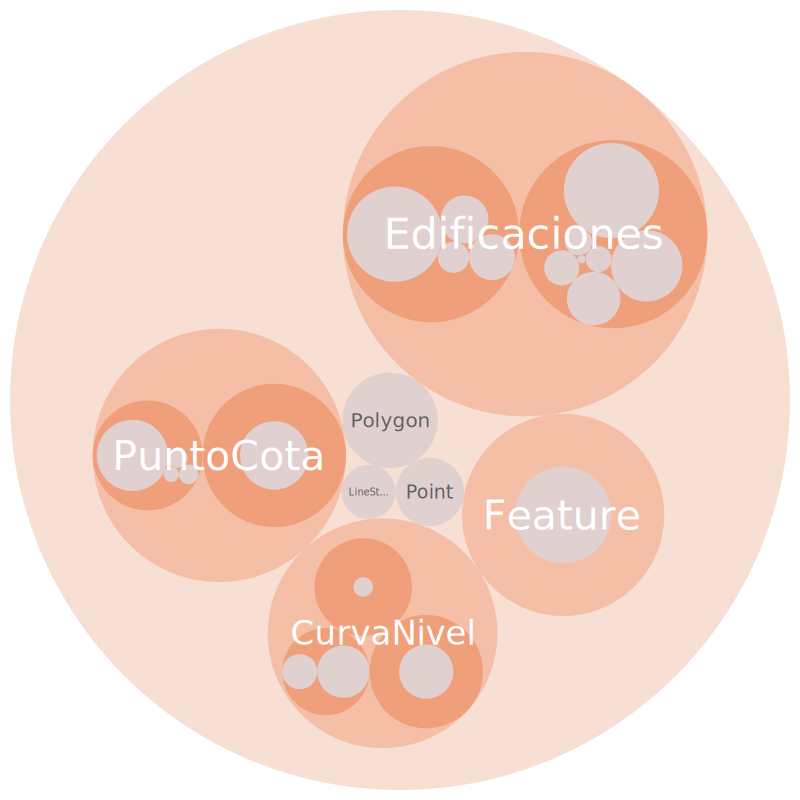
\includegraphics[width=0.7\linewidth]{imagenes/capitulo4/class-hierarchy-TFM}
	\caption{}
	\label{fig:class-hierarchy-tfm}
\end{figure}


\begin{figure}[H]
	\centering
	\includegraphics[width=0.7\linewidth]{imagenes/capitulo4/class-hierarchy-TFM-2}
	\caption{}
	\label{fig:class-hierarchy-tfm-2}
\end{figure}

\begin{figure}[H]
	\centering
	\includegraphics[width=0.7\linewidth]{imagenes/capitulo4/class-hierarchy-TFM-3}
	\caption{}
	\label{fig:class-hierarchy-tfm-3}
\end{figure}

\begin{figure}[H]
	\centering
	\includegraphics[width=0.7\linewidth]{imagenes/capitulo4/class-hierarchy-TFM-4}
	\caption{}
	\label{fig:class-hierarchy-tfm-4}
\end{figure}





Para entrar en contacto con las consultas de SPARQL y GeoSPARQL, vamos a recordar unas cuantas cosas.

Lo primero, disponemos de la información geográfica espacial referente a Ogíjares con respecto edificaciones, curvas de nivel y cotas de altura. Con esta información, que fue seleccionada para un fin, queremos saber las edificaciones que se encuentran a una cierta altura con el fin de obtener un objetivo, para ello, hemos cogido dos geometrías que nos pueden dar la misma aproximacion pero con geometrías distintas, una con puntos y otra con líneas.



\begin{lstlisting}
PREFIX rdf: <http://www.w3.org/1999/02/22-rdf-syntax-ns#>
PREFIX owl: <http://www.w3.org/2002/07/owl#>
PREFIX my: <http://example.org/ApplicationSchema#>
PREFIX geo: <http://www.opengis.net/ont/geosparql#>
PREFIX geosparql: <http://www.opengis.net/ont/geosparql#>

SELECT ?x ?p
WHERE {
?x rdf:type geo:EDI .
?polygon geo:asWKT ?p
}
LIMIT 3
\end{lstlisting}

\begin{figure}[H]
	\centering
	\includegraphics[width=0.7\linewidth]{imagenes/capitulo4/salida3}
	\caption{}
	\label{fig:salida3}
\end{figure}



\begin{lstlisting}
PREFIX rdf: <http://www.w3.org/1999/02/22-rdf-syntax-ns#>
PREFIX owl: <http://www.w3.org/2002/07/owl#>
PREFIX my: <http://example.org/ApplicationSchema#>
PREFIX geo: <http://www.opengis.net/ont/geosparql#>
PREFIX sf: <http://www.opengis.net/ont/sf#>
PREFIX xsd: <http://www.w3.org/2001/XMLSchema#>

SELECT ?f

WHERE {
?f geo:tieneCota ?fWKT
FILTER (?fWKT > 700)
}
LIMIT 5
\end{lstlisting}


\begin{figure}[H]
	\centering
	\includegraphics[width=0.7\linewidth]{imagenes/capitulo4/salida4}
	\caption{}
	\label{fig:salida4}
\end{figure}


\begin{lstlisting}
        PREFIX my: <http://example.org/ApplicationSchema#>
PREFIX geo: <http://www.opengis.net/ont/geosparql#>
SELECT DISTINCT ?point ?pointWKT ?pointCOTA
WHERE 
{
# Obtenemos todos los puntos con una cota determinada (> 720)
?point 	geo:asWKT ?pointWKT ;
geo:tieneCota ?pointCOTA .
FILTER (xsd:double(?pointCOTA) > 720)
}
LIMIT 3
\end{lstlisting}


\begin{figure}[H]
	\centering
	\includegraphics[width=0.7\linewidth]{imagenes/capitulo4/salida6}
	\caption{}
	\label{fig:salida6}
\end{figure}



Hay que tener en cuenta que hay muchas maneras de hacer las consultas, por lo que para obtener una cosa, no es necesario realizar la misma consulta,como acabamos de comprobar.

\begin{lstlisting}
PREFIX my: <http://example.org/ApplicationSchema#>
PREFIX geo: <http://www.opengis.net/ont/geosparql#>

PREFIX rdf: <http://www.w3.org/1999/02/22-rdf-syntax-ns#>

SELECT DISTINCT ?point ?pointCota
WHERE {
# Obtenemos todos los puntos con una cota determinada (> 720)
?point rdf:type geo:DEP ;
geo:tieneCota ?pointCota ;

FILTER (?pointCota > 700)
}
ORDER BY DESC(?pointCota)
LIMIT 5
\end{lstlisting}

\begin{figure}[H]
	\centering
	\includegraphics[width=0.7\linewidth]{imagenes/capitulo4/salida5}
	\caption{}
	\label{fig:salida5}
\end{figure}


\underline{GEOF:sfEquals}

\begin{lstlisting}
PREFIX my: <http://example.org/ApplicationSchema#>
PREFIX geo: <http://www.opengis.net/ont/geosparql#>
PREFIX geof: <http://www.opengis.net/def/function/geosparql/>

SELECT ?f
WHERE {
?f geo:asWKT ?fWKT .
FILTER (geof:sfEquals(?fWKT, '''
LINESTRING (440972.52 4106237.28,440972.4 4106232.04,440972.15 4106226.75,440967.68 4106204.44,440964.32 4106205.94,440963.48 4106208.23,440962.08 4106213.03,440960.59 4106219.28,440959.9 4106224.26,440958.99 4106229.78,440958.44 4106234.81,440958.11 4106240.01,440958.05 4106245.3,440958.04 4106250.86,440958.16 4106255.93,440958.41 4106261.44,440959.21 4106266.96,440960.76 4106272.24,440971.61 4106288.61,440974.39 4106281.06,440974.85 4106275.81,440974.77 4106270.3,440972.52 4106237.28)
'''^^geo:wktLiteral))
} 
\end{lstlisting}

\begin{figure}[H]
	\centering
	\includegraphics[width=0.7\linewidth]{imagenes/capitulo4/salida1}
	\caption{}
	\label{fig:salida1}
\end{figure}


\begin{lstlisting}
<!-- http://www.opengis.net/ont/geosparql#172684 -->

<owl:NamedIndividual rdf:about="http://www.opengis.net/ont/geosparql#172684">
<rdf:type rdf:resource="http://www.opengis.net/ont/geosparql#CGN"/>
<rdf:type rdf:resource="http://www.opengis.net/ont/geosparql#CMB"/>
<rdf:type rdf:resource="http://www.opengis.net/ont/geosparql#GID"/>
<rdf:type rdf:resource="http://www.opengis.net/ont/geosparql#NOR"/>
<rdf:type rdf:resource="http://www.opengis.net/ont/sf#LineString"/>
<geo:asWKT rdf:datatype="http://www.opengis.net/ont/geosparql#wktLiteral">LINESTRING (440972.52 4106237.28,440972.4 4106232.04,440972.15 4106226.75,440967.68 4106204.44,440964.32 4106205.94,440963.48 4106208.23,440962.08 4106213.03,440960.59 4106219.28,440959.9 4106224.26,440958.99 4106229.78,440958.44 4106234.81,440958.11 4106240.01,440958.05 4106245.3,440958.04 4106250.86,440958.16 4106255.93,440958.41 4106261.44,440959.21 4106266.96,440960.76 4106272.24,440971.61 4106288.61,440974.39 4106281.06,440974.85 4106275.81,440974.77 4106270.3,440972.52 4106237.28)</geo:asWKT>
<geo:tieneCota rdf:datatype="http://www.w3.org/2001/XMLSchema#double">780.0</geo:tieneCota>
</owl:NamedIndividual>
\end{lstlisting}


\begin{lstlisting}
PREFIX my: <http://example.org/ApplicationSchema#>
PREFIX geo: <http://www.opengis.net/ont/geosparql#>
PREFIX geof: <http://www.opengis.net/def/function/geosparql/>

SELECT ?f
WHERE {
?f geo:asWKT ?fWKT .
FILTER (geof:sfEquals(?fWKT, '''
POLYGON ((446050.16 4107127.71,446053.42 4107107.66,446029.09 4107103.93,446028.94 4107104.69,446027.13 4107112.67,446041.35 4107115.08,446039.91 4107125.24,446050.16 4107127.71))
'''^^geo:wktLiteral))
} 
\end{lstlisting}

\begin{figure}[H]
	\centering
	\includegraphics[width=0.7\linewidth]{imagenes/capitulo4/salida2}
	\caption{}
	\label{fig:salida2}
\end{figure}

\begin{figure}[H]
	\centering
	\includegraphics[width=0.7\linewidth]{imagenes/capitulo4/info-salida}
	\caption{}
	\label{fig:info-salida}
\end{figure}


\begin{lstlisting}
    <!-- http://www.opengis.net/ont/geosparql#181064 -->

<owl:NamedIndividual rdf:about="http://www.opengis.net/ont/geosparql#181064">
<rdf:type rdf:resource="http://www.opengis.net/ont/geosparql#EDI"/>
<rdf:type rdf:resource="http://www.opengis.net/ont/geosparql#GID"/>
<rdf:type rdf:resource="http://www.opengis.net/ont/geosparql#USO"/>
<rdf:type rdf:resource="http://www.opengis.net/ont/sf#Polygon"/>
<geo:asWKT rdf:datatype="http://www.opengis.net/ont/geosparql#wktLiteral">POLYGON ((446050.16 4107127.71,446053.42 4107107.66,446029.09 4107103.93,446028.94 4107104.69,446027.13 4107112.67,446041.35 4107115.08,446039.91 4107125.24,446050.16 4107127.71))</geo:asWKT>
</owl:NamedIndividual>
\end{lstlisting}

\underline{GEOF:WITHIN}

\begin{lstlisting}
PREFIX my: <http://example.org/ApplicationSchema#>
PREFIX geo: <http://www.opengis.net/ont/geosparql#>
PREFIX geof: <http://www.opengis.net/def/function/geosparql/>

PREFIX rdfs: <http://www.w3.org/2000/01/rdf-schema#>
SELECT ?f
WHERE {
?f geo:asWKT ?fWKT .
FILTER (geof:sfEquals(?fWKT, '''
MULTIPOINT ((446228.92 4108432.53))
'''^^geo:wktLiteral))
} 


\end{lstlisting}

\begin{figure}[H]
	\centering
	\includegraphics[width=0.7\linewidth]{imagenes/capitulo4/salida7}
	\caption{}
	\label{fig:salida7}
\end{figure}


geof:distance

Find the 3 closest features to feature my:C, where computations are based on my:hasExactGeometry.

\begin{lstlisting}
PREFIX uom: <http://www.opengis.net/def/uom/OGC/1.0/>
PREFIX my: <http://example.org/ApplicationSchema#>
PREFIX geo: <http://www.opengis.net/ont/geosparql#>
PREFIX geof: <http://www.opengis.net/def/function/geosparql/>

SELECT ?f
WHERE {
geo:889549 geo:asWKT ?WKT .
?f geo:asWKT ?fWKT .
FILTER (?fGeom != ?WKT)
}

ORDER BY ASC(geof:distance(?cWKT, ?fWKT, uom:metre))
LIMIT 5
\end{lstlisting}

\begin{figure}[H]
	\centering
	\includegraphics[width=0.7\linewidth]{imagenes/capitulo4/salida8}
	\caption{}
	\label{fig:salida8}
\end{figure}


\begin{lstlisting}
PREFIX uom: <http://www.opengis.net/def/uom/OGC/1.0/>
PREFIX my: <http://example.org/ApplicationSchema#>
PREFIX geo: <http://www.opengis.net/ont/geosparql#>
PREFIX geof: <http://www.opengis.net/def/function/geosparql/>
PREFIX rdf: <http://www.w3.org/1999/02/22-rdf-syntax-ns#>
PREFIX sf: <http://www.opengis.net/ont/sf#>

SELECT ?f
WHERE {
geo:889549 geo:asWKT ?WKT .

?f rdf:type sf:Point ;
geo:asWKT ?fWKT .
FILTER (?fGeom != ?WKT)
}

ORDER BY ASC(geof:distance(?cWKT, ?fWKT, uom:metre))
LIMIT 5
\end{lstlisting}

\begin{figure}[H]
	\centering
	\includegraphics[width=0.7\linewidth]{imagenes/capitulo4/salida9}
	\caption{}
	\label{fig:salida9}
\end{figure}

\begin{lstlisting}
PREFIX uom: <http://www.opengis.net/def/uom/OGC/1.0/>
PREFIX my: <http://example.org/ApplicationSchema#>
PREFIX geo: <http://www.opengis.net/ont/geosparql#>
PREFIX geof: <http://www.opengis.net/def/function/geosparql/>
PREFIX rdf: <http://www.w3.org/1999/02/22-rdf-syntax-ns#>
PREFIX sf: <http://www.opengis.net/ont/sf#>

SELECT ?f
WHERE {
geo:889549 geo:asWKT ?WKT .

?f rdf:type sf:LineString ;
geo:asWKT ?fWKT .
FILTER (?fGeom != ?WKT)
}

ORDER BY ASC(geof:distance(?cWKT, ?fWKT, uom:metre))
LIMIT 5
\end{lstlisting}

\begin{figure}[H]
	\centering
	\includegraphics[width=0.7\linewidth]{imagenes/capitulo4/salida10}
	\caption{}
	\label{fig:salida10}
\end{figure}

\begin{lstlisting}
PREFIX uom: <http://www.opengis.net/def/uom/OGC/1.0/>
PREFIX my: <http://example.org/ApplicationSchema#>
PREFIX geo: <http://www.opengis.net/ont/geosparql#>
PREFIX geof: <http://www.opengis.net/def/function/geosparql/>
PREFIX rdf: <http://www.w3.org/1999/02/22-rdf-syntax-ns#>
PREFIX sf: <http://www.opengis.net/ont/sf#>

SELECT ?p
WHERE {
?p rdf:type sf:Polygon ;
geo:asWKT ?pWKT .

?f rdf:type sf:Point ;
geo:tieneCota ?pointCota ;
geo:asWKT ?fWKT .

FILTER (?pointCota > 700)

}

ORDER BY ASC(geof:distance(?pWKT, ?fWKT, uom:metre))
LIMIT 5
\end{lstlisting}

\begin{figure}[H]
	\centering
	\includegraphics[width=0.7\linewidth]{imagenes/capitulo4/salida11}
	\caption{}
	\label{fig:salida11}
\end{figure}



geo:sfContains



\subsection{Visualización de la Información Geográfica}


Sin embargo, con eso sólo podemos obtener los identificadores que queremos, ¿entonces como podemos visualizarlo y ubicarlos en un mapa?

La respuesta es muy simple con Leaflet.



\section{Evaluación de la prueba de concepto}





\newpage





%Gracias a este tipo de archivo podemos generar MDT secundarios: mapas de orientación, de pendiente, cuencas visuales o sencillos archivos de sombreado (\textit{hillshade}), materia prima con la que analizar el territorio. Es por ello que, una vez descargados nuestros datos, ya podemos llevar a cabo el análisis del mapa de sombras para el MDT. Primero lo realizaremos en R, seguidamente en QGIS y, por último, veremos la interacción entre ambas, dejando documentado el proceso, para así poder hacer la evaluación y comparación entre ambas herramientas.





\newpage

% Uso de la similitud semántica para la recuperación de información geoespacial: https://dialnet.unirioja.es/servlet/tesis?codigo=61960
% http://rua.ua.es/dspace/handle/10045/45811
% https://rua.ua.es/dspace/bitstream/10045/45811/1/tesis_machado_garcia.pdf

% http://www.ciw.cl/material/tw07arodriguez.pdf

% Semántica Geoespacial en la web: https://slideplayer.es/slide/10277009/

% https://nextweb.gnoss.com/busqueda/tag/geoespacial

% Para que es para acceder a datos espaciales en la web
% http://linkedgeodata.org/OnlineAccess
% http://linkedgeodata.org/sparql

% https://www.w3.org/community/geosemweb/wiki/Main_Page
% https://en.wikipedia.org/wiki/Semantic_Geospatial_Web
% https://www.opengeospatial.org/projects/initiatives/gswie
% http://www.personal.psu.edu/faculty/f/u/fuf1/Fonseca-Sheth.pdf

% https://www.researchgate.net/publication/283801501_Geospatial_Semantic_Web
% https://www.researchgate.net/publication/300494545_Geospatial_Data_Interoperability_Geography_Markup_Language_GML_Scalable_Vector_Graphics_SVG_and_Geospatial_Web_Services
% https://www.semanticscholar.org/paper/Supporting-Frameworks-for-the-Geospatial-Semantic-Abdelmoty-Smart/e3998c31905b0d9eebaceddad5040e940caa594a
% https://www.sciencedirect.com/science/article/pii/S1570826809000468

% https://www.mdpi.com/journal/ijgi/special_issues/geospatial_semantics

% Documentos Scholar sobre "geospatial semantic web": https://scholar.google.es/scholar?q=geospatial+semantic+web&hl=es&as_sdt=0&as_vis=1&oi=scholart

% http://www.irisa.fr/LIS/ferre/sparklis/?title=Core%20English%20DBpedia&endpoint=http%3A//servolis.irisa.fr/dbpedia/sparql&sparklis-query=%5BVId%5DReturn%28Det%28An%281%2CModif%28Select%2CUnordered%29%2CClass%28%22http%3A//dbpedia.org/ontology/Database%22%29%29%2CNone%29%29&sparklis-path=D
% http://www.irisa.fr/LIS/ferre/sparklis/?endpoint=http%3A//servolis.irisa.fr/dbpedia/sparql&sparklis-query=%5BVId%5DReturn%28Det%28An%287%2CModif%28Select%2CUnordered%29%2CClass%28%22http%3A//dbpedia.org/ontology/Place%22%29%29%2CNone%29%29&sparklis-path=D

% https://www.sciencedirect.com/science/article/pii/S1570826809000468

% http://www.geonames.org/ontology/documentation.html

% https://ieeexplore.ieee.org/document/1656068

% https://www.chnt.at/the-geospatial-semantic-web-as-foundation-for-knowledge-networks-of-cultural-heritage/

% http://geoknow.eu/Welcome.html


%Un SIG ha sido ampliamente utilizado por una variedad de aplicaciones, muchas bases de datos geográficas han sido desarrolladas por diferentes programas y software. Sin embargo, sigue siendo un gran problema compartir estos datos geoespaciales y usarlos para el desarrollo de aplicaciones SIG. No es que los datos no estén disponibles, hay una gran cantidad de datos geográficos almacenados en diferentes lugares y en diferentes formatos, pero la reutilización de datos para nuevas aplicaciones y el intercambio de datos son tareas abrumadoras debido a la heterogeneidad de los sistemas existentes en términos de conceptos de modelado de datos, técnicas de codificación de datos y estructuras de almacenamiento, etc.\\

%Hay dos problemas que resultan directamente de la no interoperabilidad de las bases de datos. Uno es el cambio en la exactitud de los datos. Después de que los datos se conviertan de un formato a otro, pueden ocurrir problemas como la precisión de coordenadas, errores de omisión, nombres de atributos faltantes o incorrectos y una topología incorrecta. El segundo problema es la inversión de tiempo y dinero para la conversión de datos. Se ha desperdiciado mucho dinero y tiempo en la conversión de datos o en el desarrollo de herramientas de conversión de datos.\\

%La interoperabilidad de datos significa la capacidad de utilizar una variedad de formatos de datos. Los datos geoespaciales interoperables pueden ser utilizados por diferentes tipos de programas y aplicaciones. Con datos geoespaciales interoperables, los usuarios deben poder solicitar, acceder e integrar datos fácilmente sin importar dónde se almacenen los datos (local o remotamente). La interoperabilidad de los datos geoespaciales es extremadamente importante para las aplicaciones geoespaciales, ya que existían grandes cantidades de datos espaciales de diferentes formatos geográficos y hay una mayor demanda de reutilización de estos datos espaciales existentes para la toma de decisiones. La interoperabilidad de los datos geoespaciales elimina las barreras para el intercambio de datos y permite a los usuarios acceder, mapear, visualizar y analizar directamente datos con diferentes formatos de datos espaciales. Los datos geoespaciales interoperables hacen posible la distribución rápida de información y el intercambio entre departamentos.\\


%\section{Web Semántica Geoespacial}

% http://www.mclibre.org/consultar/xml/lecciones/web-semantica.html#spatial-data

%\subsection{Arquitectura Web Semántica Geoespacial}

% se debería de hacer una mención a la web semántica tradicional o la web tradicional


% 

https://mangomap.com/gis-mapping

% ---------------------------------------------------------------------------

%¿qué datos cogemos?
%
%Descargamos datos de aquí: https://www.juntadeandalucia.es/institutodeestadisticaycartografia/bcadescargas/
%- Base Cartográfica de Andalucía (2) > Base Cartográfica de Andalucía (shape) > Ogíjares
%
%Para saber más información acerca de los datos: https://www.juntadeandalucia.es/institutodeestadisticaycartografia/prodCartografia/bc/modelo.htm
%
%Para instalar Google Maps en QGIS
%https://mappinggis.com/2018/03/como-anadir-mapas-base-en-qgis-3-0-openstreetmap-google-carto-stamen/
%
%
%- Elemento Edificaciones (poligonal): Se agrupan en esta capa varios elementos que conforman edificaciones. Se debe tener en cuenta que el nucleo urbano engloba en áreas grandes a las edificaciones.
%
%- Elemnto ParqueJardinP (puntual): Recinto en el interior de una población destinado a prados, jardines y arbolado
%para recreo y ornato. 

%-----

%Se trabajará con información  geoespacial, concretamente con archivos en formato Shapefile. 
%
%La mejora de las herramientas se enfocará únicamente a las destinadas a la generación (QGIS que permitirá llevar la información  de los shapefile hacia hojas de cálculo y Protegé permitirá llevar la información  de los shapefile hacia documentos en formato RDF), y consumo GraphBD que permite la visualización de archivos en formato RDF y visualización (aplicación en R que permite la visualización de archivos en formato RDF),  y como lenguaje de consulta geoespacial, este estándar es GEOSPARQL.
%
%Finalmente, todos los datos generados mediante las herramientas mejoradas, se publicarán en un repositorio disponible, el cual dará lugar al: repositorio de Datos Enlazados Ecuatoriano el cual debe permitir su acceso al público en general. 


% ----

%Para hacer uso de este lenguaje de consulta, es necesario utilizar herramientas que permitan GeoSPARQL, no sólo SPARQL. Es por eso que la herramienta Protegé carece de funcionamiento para este tipo de consultas
%
%Como hemos comentado anteriormente, la herramienta Protegé nos permite construir contologías de manera más sencilla y rápida, sin embargo, también nos ofrece herramienta para realizar consultas con SPARQL. No obstante, carece de funcionamiento para las consultas de GeoSPARQL. En el siguiente apartado, hablaremos también 
%
%en este caso, 

%---

\section{Resumen del capítulo}





